% Copyright (C) 2005-2015 Airbus - EDF - IMACS - Phimeca
% Permission is granted to copy, distribute and/or modify this document
% under the terms of the GNU Free Documentation License, Version 1.2
% or any later version published by the Free Software Foundation;
% with no Invariant Sections, no Front-Cover Texts, and no Back-Cover
% Texts.  A copy of the license is included in the section entitled "GNU
% Free Documentation License".
\renewcommand{\nomfichier}{docref_C312_SampleSphere}
\renewcommand{\titrefiche}{Sphere sampling method}

\Header

\MathematicalDescription{
  \underline{\textbf{Goal}} \vspace{2mm}

  Within the context of the First and Second Order of the Reliability Method (refer to \otref{docref_C311_Form}{FORM} and \otref{docref_C311_Sorm}{SORM}), the Strong Maximum Test (refer to \otref{docref_C312_StrongMaxTest}{Strong Maximum Test}) helps to check whether the design point computed is :
  \begin{itemize}
  \item the true design point, which means a global maximum point,
  \item a strong design point, which means that there is no other local maximum verifying the event and associated to a value near the global maximum.
  \end{itemize}

  The Strong Maximum Test samples a sphere in the standard space. OpenTURNS standard version uses the gaussian random sampling technique described hereafter.
  \vspace{2mm}

  \underline{\textbf{Principle}} \vspace{2mm}

  OpenTURNS standard version uses the gaussian random sampling technique:
  \begin{enumerate}
  \item sampling of points in $\Rset^N$ according to a radial distribution : we generate  $N$ independent standard normal samples,
  \item  projection of the points onto $\cS^{*}$ : we map the points different from the origin using the transformation $M\longmapsto m$ such as $\displaystyle\mathbf{Om}=R\frac{\mathbf{OM}}{\|\mathbf{OM}\|}$ where $R$ is the radius of the sphere of interest. This transformation does not depend on the angular coordinates. Thus, the generated points follow a uniform distribution on $\cS^{*}$.
  \end{enumerate}

  A result of such an algorithm is drawn on the following figure \ref{figstoch2}.
  \begin{center}
    \resizebox{6cm}{6cm}{\label{figstoch2}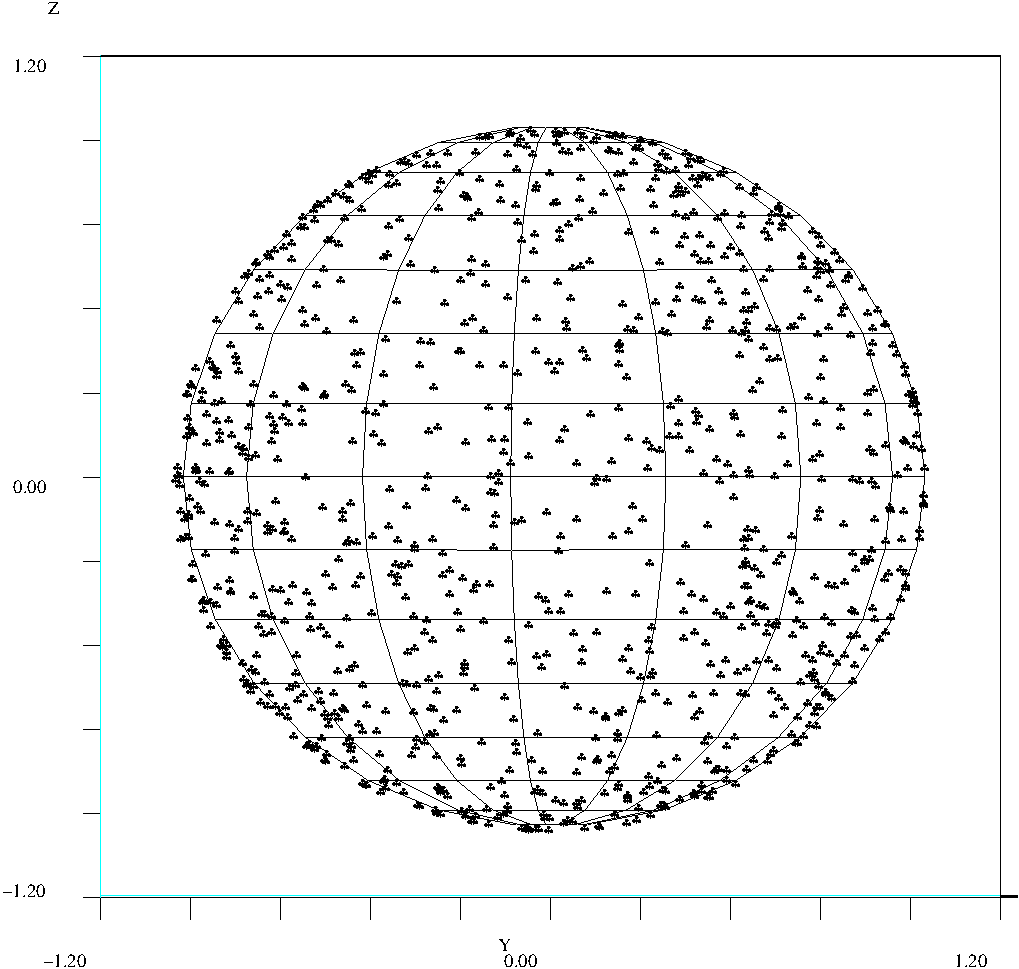
\includegraphics{Figures/AleaGauss.pdf}}
    % \caption{Stochastic sampling of $\cS_3$ : gaussian method.}
    % \label{figstoch2}
  \end{center}
}
{
  -
}

\Methodology{
  Within the global methodology, the sphere sampling method  is used in the step C, within the Strong Maximum Test (refer to \otref{docref_C312_StrongMaxTest}{Strong Max Test}).\\
  It requires to have fulfilled the following steps beforehand:
  \begin{itemize}
  \item step A: identify of an input vector $\vect{X}$ of sources of uncertainties and an output variable of interest $Z=\tilde{g}(\vect{X},\vect{d})$, result of the model $\tilde{g}()$; identify a probabilistic criteria such as a threshold exceedance $Z > z_s$ or equivalently a failure event ${g(\vect{X}\,,\,\vect{d}) \le 0}$,
  \item step B: identify one of the proposed techniques to estimate a probabilistic model of the input vector $\vect{X}$,
  \item step C: select an appropriate optimization algorithm among those proposed to evaluate the Form or Sorm approximations of $P_f$; evaluate the quality of the design point resulting from the previous step thanks to the Strong Maximum Test.
  \end{itemize}
}
            {
              Other methods can be used to sample the hypersphere of dimension $N-1$ in $\Rset^N$ : the exclusion method and the parametric method.\\
              The parametric method uses the polar coordinates : the angle parameters are discretized uniformly. It has the inconvenient to generate points principally in the two poles zones.\\
              The exclusion method generates points uniformly within the hypercube containing exactly the sphere. Then we keep only the points located inside the sphere, and we project them on the sphere. This method has the inconvenient to be inefficient for high dimensions : the fraction between the  volume of the hypersphere and the volume of the hypercube  is less than $0.7 \%$ as soon as the dimension is greater than 9. Il means that for a dimension greater than 9, $99.3\%$ of the points generated are rejected. \\

              Let's note some usefull references:
              \begin{itemize}
              \item Luban, Marshall, Staunton, 1988, "An efficient method for generating a uniform distribution of points within a hypersphere," Computer in Physics, 2(6), 55.
              \end{itemize}
            }
